\chapter{Primzahlen, RH und die Musik hinter den Schatten}
\label{ch:shadow-arithmetic}
\begin{bild}{Was uns ein Schatten verraten kann}
Wenn wir nur den Schatten eines Rades sehen, erkennen wir vielleicht einen Kreis. Erst wenn wir das Rad drehen, belasten und mit einem zweiten Rad verbinden, erkennen wir seine Achse, seine Zähne und seine Übersetzung. Genau so lesen wir hier Primzahlen, Quanteneffekte und Raumzeit: als verschiedene Antworten, die eine mögliche gemeinsame Struktur gleichzeitig erklären müsste.
\end{bild}

Die folgenden fünf Kapitel erweitern die ursprüngliche Synthese. Sie verbinden den verfügbaren RH- und Primzahlenzweig mit externer Primärliteratur und eigenen Gegenrechnungen. Dabei bedeutet \emph{Schatten} je nach Stelle etwas Genaues: eine Zählfolge, eine Spur, ein Spektrum, eine Messstatistik oder eine reduzierte Dynamik. Erst ein angegebener Übersetzungspfeil macht aus einer Ähnlichkeit eine mathematische Verbindung.

\section{In welchem Sinn Primzahlen Bausteine sind}
Jede natürliche Zahl $n>1$ zerfällt eindeutig in Primfaktoren:
\begin{equation}
 n=\prod_p p^{\nu_p(n)},\qquad \log n=\sum_p\nu_p(n)\log p.
\end{equation}
Die erste Gleichung beschreibt ein Zusammensetzen durch Multiplikation; die zweite übersetzt dieses Zusammensetzen in Addition. Zum Beispiel ist $360=2^3\cdot3^2\cdot5$, also $\log360=3\log2+2\log3+\log5$. Die Primzahlen sind die unabhängigen Bausteine dieses \emph{multiplikativen} Systems. Das ist ein Satz über natürliche Zahlen. Es ist noch kein Satz darüber, dass Elektronen aus Primzahlen bestehen.

Ein hilfreiches physikalisches Modell liest die Exponenten $\nu_p$ als Besetzungszahlen von Moden mit Energien $E_p=E_*\log p$. Dann entspricht jeder Gesamtzustand genau einer Zahl $n$ und hat Energie $E_*\log n$. Mit dimensionsloser inverser Temperatur $\beta=E_*/(k_BT)$ ergibt sich
\begin{equation}
 Z(\beta)=\sum_{n\geq1}n^{-\beta}
 =\prod_p\frac1{1-p^{-\beta}}=\zeta(\beta),\qquad \beta>1.
 \label{eq:primon-partition}
\end{equation}
Das bosonische Besetzungsmodell erlaubt beliebig viele Exemplare jedes Primbausteins. Beschränkt man jede Primzahl auf null oder eins, entsteht stattdessen $\zeta(\beta)/\zeta(2\beta)$. Mit zusätzlichem Vorzeichen $(-1)^{\text{Besetzungszahl}}$ entsteht $1/\zeta(\beta)$. Die Statistik und die gewählte Spur entscheiden also darüber, \emph{welcher} arithmetische Schatten erscheint. \src{R09; F03}

Das Bost--Connes-System macht aus solchen arithmetischen Zutaten eine ausgearbeitete Quantenstatistik mit einer Algebra, Zeitentwicklung und Gleichgewichtszuständen. Seine Phasenstruktur ist ein mathematisches Ergebnis dieses Systems. Weder seine Existenz noch seine Zetafunktion als Zustandssumme beweist RH oder identifiziert ein bereits natürlich realisiertes TFPT-System. \src{F03}

\subsection{Eine bedingte Auswahlregel für die logarithmische Energie}
Warum gerade $\log n$? Aus $e(mn)=e(m)+e(n)$ allein folgt das noch nicht: Man darf jeder Primzahl zunächst einen beliebigen Wert $e(p)$ geben. Eine zusätzliche Ordnungsregel schließt die Lücke. Ist $e$ monoton in der natürlichen Zahl $n$, so gilt notwendig
\begin{equation}e(n)=c\log n,\qquad c\geq0.\end{equation}
Der Beweis ist kurz. Setze $k=\lfloor\ell\log_2n\rfloor$. Aus $2^k\leq n^\ell<2^{k+1}$ folgen
\[
 k\,e(2)\leq\ell\,e(n)\leq(k+1)e(2).
\]
Division durch $\ell$ und der Grenzübergang $\ell\to\infty$ ergeben $e(n)=e(2)\log_2n$. Das ist eine elementare mathematische Auswahlregel, hier als Anschlussargument verwendet. Sie leitet die physikalische \emph{Gültigkeit der Monotonie} und die Energieskala $E_*$ nicht aus TFPT ab.

Im vorhandenen Entropiezweig liefert die Kreisabbildung $x\mapsto mx\pmod1$ die Periodenpunktzahl $m^k-1$ und die Wachstumsentropie $\log m$. Damit ist eine natürliche logarithmische Größe vorhanden. Die Gleichsetzung dieser Entropie mit einer Hamiltonenergie bleibt eine zusätzliche Zuordnung; die Kreisabbildung ist zunächst eine nichtinvertierbare Überlagerung. \src{R10}

\section{Was Primzahlen mit Quantenchaos verbindet}
Die häufig verkürzte Aussage \glqq Primzahlen tauchen als Quantenenergien auf\grqq{} umfasst verschiedene Sachverhalte. Beim klassischen Zeta--Quantenchaos-Vergleich entsprechen \emph{Nullstellenhöhen} den Energien eines gesuchten Spektrums. Die Primzahlen spielen auf der anderen Seite die Rolle \emph{primitiver periodischer Bahnen}; Primzahlpotenzen sind deren Wiederholungen. Eine Bahn wird einmal durchlaufen, zweimal, dreimal. Ihr logarithmischer Takt ist $\log p$. \src{F01}

Die exakte Ausgangsidentität lautet
\begin{equation}
 -\frac{\zeta'(s)}{\zeta(s)}
 =\sum_p\sum_{r\geq1}(\log p)\,p^{-rs},\qquad\Re s>1.
 \label{eq:prime-trace}
\end{equation}
Sie folgt durch logarithmisches Ableiten des Eulerprodukts. Beim Übergang zur Nullstellenseite treten die glatten, archimedischen und Polbeiträge hinzu. Die oft gezeichnete oszillierende Dichte mit Termen $-(\log p)p^{-r/2}\cos(tr\log p)/\pi$ ist auf der kritischen Geraden \emph{keine gewöhnlich konvergente Punkt-für-Punkt-Reihe}; sie braucht eine präzise Glättung oder distributionelle Lesart.

\begin{figure}[H]\centering
\begin{tikzpicture}[node distance=8mm]
\node[box,text width=39mm] (a) {Primzahl $p$\\primitiver Baustein};
\node[box,text width=39mm,right=8mm of a] (b) {$p^r$ und $r\log p$\\Wiederholung};
\node[box,text width=39mm,right=8mm of b] (c) {Explizite Formel\\mit allen Beiträgen};
\node[openbox,text width=91mm,below=12mm of b] (d) {Nullstellen als Spektrum\\Gesuchte selbstadjungierte Realisierung und exakte Identifikation bleiben offen};
\draw[arr] (a)--(b);\draw[arr] (b)--(c);\draw[hyp] (c.south) |- (d.east);
\end{tikzpicture}
\caption{Die arithmetische Übersetzung ist konkret. Der Schritt zu einem nativen physikalischen Spektrum benötigt mehr als ähnliche Abstände.}
\end{figure}

Odlyzkos Nullstellenrechnungen zeigen sehr genaue Übereinstimmung mit den Abstandsstatistiken der GUE; Montgomerys bewiesene Paar-Korrelation besitzt zusätzliche Voraussetzungen und einen beschränkten Testbereich. Die vollständige statistische Aussage ist umfassender. GUE bezeichnet die Klasse ohne eine passende Zeitumkehrsymmetrie; andere Quantensysteme zeigen andere Klassen. Arithmetische Quantisierungen können außerdem zusätzliche Hecke-Symmetrien besitzen. \src{F01, F02, F05}

\textbf{Die Folgerung für uns:} Eine Übereinstimmung der Zweipunktstatistik ist ein Hinweis auf eine mögliche Spektralorganisation. Sie identifiziert weder die Primzahlen einzeln noch die ganze Dynamik, ihre lokalen Observablen oder die Lage sämtlicher Nullstellen. Die arithmetischen Phasen und höheren gemeinsamen Beziehungen bleiben zusätzliche Information.

Auch das Vorzeichen ist lehrreich. Ein Ansatz, der jede primitive Bahn mit nur einer skalaren Phase $q$ versieht und für \emph{jede} Wiederholung das Vorzeichen $-1$ benötigt, scheitert bereits an $r=1,2$: Aus $q=-1$ folgt $q^2=+1$. Dieser kleine Einwand widerlegt nur diesen speziellen Ansatz. Er motiviert reichere Spuren, Gradierungen oder relative Beiträge; Connes untersucht etwa eine Absorptionsinterpretation. \src{F04; eigene algebraische Gegenprobe}

\section{Was unser RH-Zweig tatsächlich beigetragen hat}
Die Unterlagen und der zusätzlich eingesehene Forschungsbestand ergeben keine abgeschlossene RH-Lösung. Sie ergeben jedoch eine ungewöhnlich präzise Landkarte aus positiven Bausteinen und bereits ausgeschlossenen Abkürzungen. Die folgende Verdichtung ordnet die inhaltlichen Familien; sie behauptet keine erneute Prüfung jedes Katalogeintrags.

\begin{longtable}{L{31mm}L{58mm}L{59mm}}
\toprule\textbf{Zweig}&\textbf{Was vorliegt}&\textbf{Was dadurch noch fehlt}\\\midrule\endhead
$E_8$, Theta, Hecke&Die Schalenfolge $N(2n)=240\sigma_3(n)$ verbindet die Geometrie mit einem Eulerprodukt. Markierte Nachbaroperationen tragen Hecke-Daten.&Eine positive Gitterzählung ist nicht bereits das positive Weil-Funktional für alle Tests. Die arithmetische Markierung gehört zur Eingabe.\\
Gauß-/Viererstruktur&Komplexe Markierung und Restklassen können den Zweig mit $\Z[i]$ und $\chi_{-4}$ verbinden.&Eine interne $\mu_4$-Phase allein identifiziert noch keinen arithmetischen Charakter. $\chi_{-4}$ ist quadratisch und hat Leiter 4.\\
W1: Wörterbuch&Explizite Identifikation von Maß, Schraubenfunktion und arithmetischen Beiträgen; Ursprungsterm und Pole sind wesentlich.&Aus einer passenden Form einer Darstellung folgt ihre Positivität nicht automatisch.\\
W3: Detektor&Exakte Testkerne, diskrete Koeffizienten und kontrollierte Positivitätsfragen.&Positivität eines Kerns auf reellen Argumenten darf nicht voraussetzen, dass sämtliche Nullstellenargumente reell sind.\\
Toeplitz und mehrere Skalen&Schur-Komplemente und Residuen liefern unter benannten Voraussetzungen schärfere Schranken.&Endliche Fenster, gewählte Paritätssektoren und bereits vorausgesetzte Positivität ersetzen keinen vollständigen Grenzwertbeweis.\\
GUE und Ablationen&In den untersuchten Beispielen sind kohärente Aufhebungen wesentlich; Eingriffe in den Primkamm prüfen die Weltabhängigkeit.&Ein günstiger Quotient, ein Zweipunktmodell oder ein unpassendes Ersatz-Wörterbuch ist keine neue RH-Positivität.\\
Multiplikative Relationen&Multiplikativität lässt sich als Flachheit auf einem Relationskomplex ausdrücken; die ganzzahlige Randidentität ist exakt.&Die untersuchte Krümmungsdiagnose unterscheidet Varianten, liefert aber noch nicht das benötigte positive signierte Restglied.\\
Jensen/Coxeter, Selberg-Kontakt&Konkrete Strukturfehler wurden sichtbar: starres $E_8$-Spektrum versus veränderliche Jensen-Daten; falsche Positivitätsart oder Vorzeichen.&Die negativen Kontrollen gelten für die geprüften Brücken, nicht gegen alle Spektral- oder Selberg-Ansätze.\\
Faktorisierung&Zähl- und Inversionsidentitäten, modulare Dynamiken, Regulator- und Relationenansätze.&Eine leicht invertierbare Kennzahl kann selbst schwer auszulesen sein. Kosten in $N$ sind von Kosten in $\log N$ zu unterscheiden.\\\bottomrule
\end{longtable}
\src{R01--R15; ausgewählte Originalabschnitte und Ergebnisdateien}

\subsection{Der genaue Ertrag der $E_8$-Schalen}
Die ersten sechs Werte sind $240$, $2160$, $6720$, $17520$, $30240$ und $60480$. Daraus folgt für $\Re s>4$
\begin{equation}
 \sum_{n\geq1}\frac{N(2n)}{n^s}=240\zeta(s)\zeta(s-3),
 \qquad\mathop{\mathrm{Res}}_{s=4}=\frac{8\pi^4}{3}.
\end{equation}
Hier ist der Primzahlbezug wirklich vorhanden. Die Selbstdualität des Gitters schließt die Poisson-Transformation auf dasselbe Gitter. Poisson-Summation gilt auch für nichtselbstduale Gitter und verbindet dann Gitter und Dualgitter. Die geschlossene Symmetrie ist daher stärker als ein Bild, aber schwächer als RH. \src{R04}

Eine elementare Gegenprobe macht die fehlende Folgerung sichtbar:
\begin{equation}
 g(s)=\bigl((s-\tfrac34)^2+1\bigr)\bigl((s-\tfrac14)^2+1\bigr)
 =g(1-s).
\end{equation}
Trotz der Spiegelung liegen alle vier Nullstellen bei $\tfrac14\pm i$ und $\tfrac34\pm i$, also neben der Mittellinie. Dieses Polynom ist keine Ersatz-Zetafunktion: Es zeigt gezielt, dass Spiegelung \emph{allein} den Schluss nicht trägt.

\subsection{Warum die fehlende Positivität so hartnäckig ist}
Die entscheidende arithmetische Form enthält eine Differenz: vereinfacht $W=\text{Pol}+\text{Archimedes}-\text{Primbeitrag}$. Zwei positive Matrizen können eine indefinite Differenz besitzen; schon $I-\operatorname{diag}(2,0)$ hat die Eigenwerte $-1$ und $1$. Entsprechend löst ein beliebiger positiver Born- oder Gramkern die signierte Aufgabe noch nicht.

Auch die Zusammensetzung positiver Teile ist eine eigene Bedingung. Für
\[
 A=\begin{pmatrix}B&C\\C^\dagger&D\end{pmatrix},\quad B>0,
 \qquad A\succeq0\ \Longleftrightarrow\ D-C^\dagger B^{-1}C\succeq0
\]
ist der gemischte Block $C$ entscheidend. Die Diagonalblöcke der Matrix $\left(\begin{smallmatrix}1&2\\2&1\end{smallmatrix}\right)$ sind positiv; die Gesamtmatrix besitzt trotzdem den Eigenwert $-1$. Genau diese Art fehlender gemeinsamer Kontrolle verbindet das RH-Problem mit der Universalraum-Rekonstruktion: Richtige Einzelansichten bestimmen ihre Verträglichkeit noch nicht. \src{R05--R08; eigene Gegenbeispiele}

In W3 hat das Nullstellenargument die Form $\gamma_\rho=(\rho-1/2)/i$. Es ist nur dann reell, wenn die jeweilige Nullstelle auf der kritischen Geraden liegt. Die Nichtnegativität eines sinc-/Betragsquadrat-Kerns für reelles $\gamma$ darf deshalb nicht unbemerkt für alle $\rho$ benutzt werden. Ein ganzer ungerader Testsektor ist außerdem nicht mit dem gesamten mittelwertfreien Testraum gleichzusetzen. \src{R06}

\subsection{Was die negativen Routen konkret lehren}
Der Jensen/Coxeter-Test r618 findet eine starre $\Phi_{30}$-Struktur auf der $E_8$-Seite, während die verglichenen Jensen-Polynome mit ihrem Index variieren. Die gewählte Identifikation scheitert. Der Selberg-Kontakttest r638 besitzt im untersuchten Fall weiterhin einen negativen kleinsten Eigenwert von ungefähr $-0{,}003895$; eine Quadratvervollständigung hat die falsche signierte Form nicht geheilt. \src{R13, R15}

Die GUE-Ablation berichtet in ihrer gewählten endlichen Auswertung starke kohärente Auslöschungen. Eine inkohärente Abschätzung überschätzt den Bedarf erheblich. Das ist ein Hinweis, die \emph{relativen Phasen und Relationen} weiterzuführen. Es ist keine universelle gemessene Konstante und kein Nachweis unbekannter physikalischer Primwellen. Bei veränderter Primfolge muss zuerst geklärt werden, ob überhaupt dieselbe explizite Formel auf der Gegenseite existiert. \src{R11}

Im Faktorisierungszweig gilt für die untersuchte $E_8$-Gaußsumme $S_N(t)=N^4\gcd(t,N)^4$. Bestimmte daraus gebaute Zählwerte erlauben bei zugesichertem $N=pq$ eine exakte Inversion. Die direkte Baum-/Uhrauslesung bleibt aber von Größenordnung $N^3$ mit Bindungsdimension $N$. Damit ist die Inversion kein nachgewiesener schneller Algorithmus in der Eingabelänge $\log N$. Der Befund r640 \glqq kein billigerer Weg\grqq{} betrifft vier implementierte Auslesungen; er ist kein allgemeiner Unmöglichkeitssatz. Regulator-Sprünge behalten ihre Regulatorberechnung als Kosten, Relationenmethoden ihre Glattheitssuche. \src{R01, R14}

\section{Die Naht braucht mehr als ein paar zusätzliche Takte}
Die vorhandene freie fermionische Naht hat bei fester Größe eine endliche Zustandssumme. Das Primonmodell verlangt eine unbegrenzte Primfamilie und andere Besetzungsdaten. Schon für $\{2,3,5\}$ gilt $Z(1)=15/4$ und $Z(2)=25/16$: Der Pol bei $\beta=1$ entsteht erst in der unendlichen Familie. Eine endliche Demonstration kann ihn nicht besitzen. Der vorhandene Nahtvergleich findet entsprechend keine vollständige Identifikation. Ein anders aufgebauter Grenzwert einer wachsenden Familie wird dadurch nicht ausgeschlossen. \src{R09}

\Needspace{180pt}
\begin{grenze}{Ein präzises Hindernis für ein endliches additives Uhralphabet}
Angenommen, sämtliche primitiven Perioden eines Modells liegen in der ganzzahligen linearen Hülle von endlich vielen festen Takten $\tau_1,\ldots,\tau_r$. Dann können diese Perioden nicht alle Zahlen $\log p$ umfassen.

Denn aus $\sum_{j=1}^m a_j\log p_j=0$ mit rationalen $a_j$ folgt nach Nennerbeseitigung $\prod p_j^{b_j}=1$. Die eindeutige Primfaktorzerlegung erzwingt $b_j=0$. Die Primlogarithmen sind also über $\mathbb Q$ linear unabhängig, während $r$ Takte höchstens einen $r$-dimensionalen rationalen Raum erzeugen.
\end{grenze}
Der konkrete Zweig hatte bereits Takte aus $\log2$ und $\log3$ gegenüber dem fehlenden $\log5$ abgegrenzt. Das Argument oben verdichtet dies zu einer allgemeinen \emph{bedingten} Aussage. Es widerlegt keine endliche Rechenregel, die beliebig viele Primzahlen generiert, und keine Dynamik mit nichtadditiven oder zustandsabhängigen Bahnzeiten. Es sagt genau, welche einfache Uhrvorstellung nicht ausreicht. \src{R10; hier ausgeschriebener Beweis}

\section{Die neue Quantenphasen-Arbeit von 2026}
Wei und Mitautoren verbinden in zwei gezielt konstruierten Quantensystemen Nullstellen mit dynamischen Phasenübergängen. Berichtet werden ein Fünf-Qubit-NMR-Prinzipversuch und weitergehende numerische Untersuchungen. Die verwendeten Hamiltonoperatoren und Zustandsgewichte sind so gewählt, dass sie Zeta-Daten kodieren. Das macht den Zusammenhang experimentell bearbeitbar; eine Ableitung dieser Wahl aus TFPT oder ein RH-Beweis folgt daraus nicht. \src{F06, veröffentlicht 1. Juli 2026}

\subsection{Eigene Anschlussrechnung: Ein verschwindendes Signal ist mehrdeutig}
Unabhängig vom vollständigen Ressourcenbeweis dieser Arbeit untersuchen wir den folgenden einfachen thermischen Eta-Auslesekanal:
\begin{equation}
 A_N(\beta,t)=\frac{\sum_{n=1}^{N}(-1)^{n-1}n^{-\beta-it}}{Z_N(\beta)},
 \qquad Z_N(\beta)=\sum_{n=1}^{N}n^{-\beta}.
 \label{eq:eta-readout}
\end{equation}
Er entsteht durch einen Gibbszustand für $\log n$ und eine diagonal ausgelesene Paritätsphase. Bei \emph{festem} $t$ und $0<\beta<1$ konvergiert der Zähler gegen $\eta(\beta+it)$, während
\[
 Z_N(\beta)\sim\frac{N^{1-\beta}}{1-\beta}.
\]
Also geht das Rohsignal $A_N$ an \emph{jedem festen} $t$ gegen null, auch ohne Zeta-Nullstelle. Innerhalb des offenen kritischen Streifens teilen $\eta(s)=(1-2^{1-s})\zeta(s)$ und $\zeta(s)$ ihre Nullstellen. Sichtbar wird diese Unterscheidung aber erst nach kontrollierter Rückskalierung und Fehlerrechnung.

\begin{figure}[H]\centering
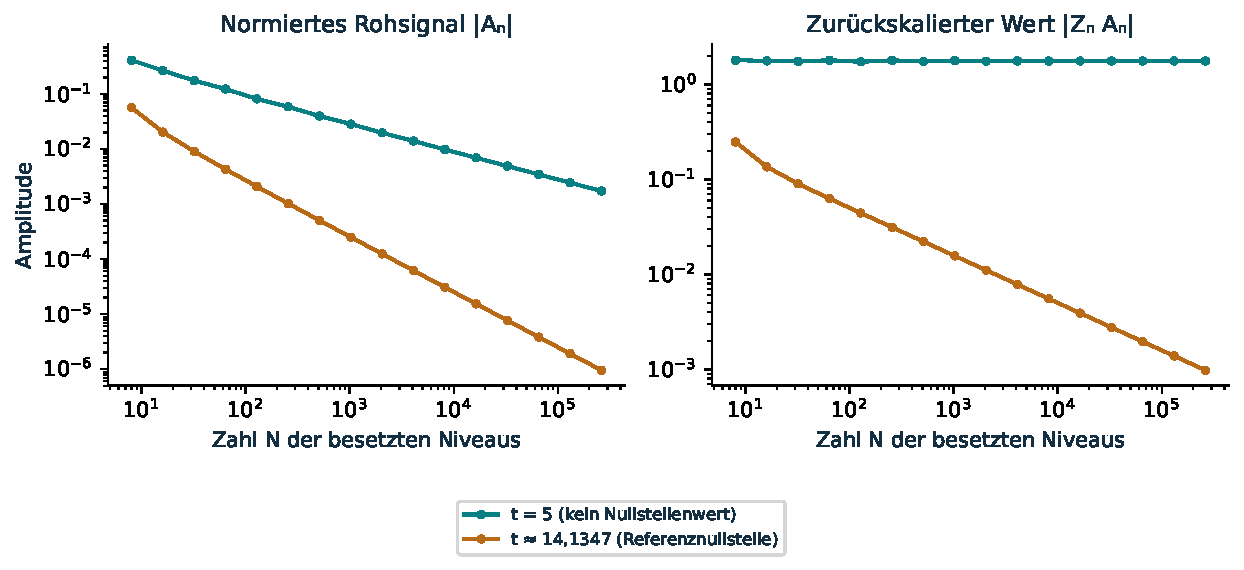
\includegraphics[width=\linewidth]{figures/shadow_eta_normalization.pdf}
\caption{Eigene endliche Rechnung für $\beta=1/2$. Links verschwinden beide Rohsignale. Rechts trennt die Rückskalierung einen gewöhnlichen Wert von der Umgebung der ersten bekannten Nullstelle. Die Kurven sind Formelauswertungen, keine Messdaten und kein Nullstellenzertifikat.}
\end{figure}

Um die zurückskalierte Amplitude mit absolutem Fehler $\varepsilon$ zu bestimmen, muss der Rohfehler von Größenordnung $\varepsilon/Z_N$ sein. Bei gewöhnlichen unabhängigen Messungen beschränkter Observablen führt die übliche Stichprobenschranke zu einem Aufwand $O(Z_N^2/\varepsilon^2)$ für feste Konfidenz. Bei $\beta=1/2$ wächst dieser wie $O(N/\varepsilon^2)$. Für $N=2^q$ ist das exponentiell in den Registerbits $q$. Dies ist eine Kostenrechnung für \emph{diesen Messweg}, keine allgemeine Quantenuntergrenze und keine Widerlegung der zwei vollständigen Protokolle von F06. Kohärente Amplitudenschätzung, andere Normierungen und gekoppelte Grenzwerte müssen jeweils separat bilanziert werden.

Der konkrete Gewinn für unser Puzzle lautet: \emph{Die Zustandsnormierung gehört zur physikalischen Bedeutung eines arithmetischen Schattens.} Registergröße, Präparation, Präzision, Messwiederholungen und Grenzwert dürfen nicht hinter einer eindrucksvollen Nullstelle verschwinden.
